\documentclass[12pt,a4paper,onecolumn]{article}
\usepackage[utf8]{inputenc}
\usepackage[portuguese]{babel}
\usepackage[T1]{fontenc}
\usepackage{graphicx}
\usepackage{amsmath,amssymb,amsthm,amsfonts}
\usepackage{setspace}
\usepackage{listings}
\usepackage{gensymb}
\usepackage{float}
\usepackage{mathtools}
% \usepackage{undertilde}

\DeclarePairedDelimiter\abs{\lvert}{\rvert}
\DeclarePairedDelimiter\norm{\lVert}{\rVert}

\makeatletter
\let\oldabs\abs
\def\abs{\@ifstar{\oldabs}{\oldabs*}}
%
\let\oldnorm\norm
\def\norm{\@ifstar{\oldnorm}{\oldnorm*}}
\makeatother

\title{Comparação de Algoritmos para Multiplicação de Matrizes}
\date{}
\author{Fernando Maciel Motta}

\begin{document}
\setcounter{section}{1}
%\begin{titlepage}
\maketitle
%\thispagestyle{empty}
%\begin{center}
%{\large Sugestão 2}\\[0.2cm]
%\end{center}
%\end{titlepage}

\onehalfspacing

\section*{Introdução}

O objetivo deste trabalho é comparar o tempo computacional gasto por diferentes algoritmos para multiplicação de matrizes.
Em particular será comparada a implementação da biblioteca BLAS, que utiliza uma versão altamente otimizada para a arquitetura do processador do método
de 3 \emph{loops}, com uma implementação em C do algoritmo de Strassen.

Teoricamente, o tempo computacional assintótico gasto pelo método de 3 \emph{loops} é $O(n^3)$, para uma matriz $n \times n$, enquanto o método de Strassen
tem tempo assintótico de $O(log_2(7) \approx O(2.81)$. Apesar disso, o método de Strassen tem um \emph{overhead} grande e se torna ineficiente para matrizes
pequenas \cite{Demmel, Pan}.

\section*{Teste de Tempo de Execução}

O método de Strassen em sua forma original só é adequado para matrizes de ordem $2^k \times 2^k$. Isto ocorre porque a sua implementação envolve dividir a matriz em 
blocos de tamanho $n/2 \times n/2$ recursivamente até chegar a blocos de tamanho $1 \times 1$ que são multiplicados trivialmente \cite{Strassen}. Para solucionar esta
limitação, duas abordagens são sugeridas.

A primeira abordagem é o \emph{Static Padding}, que envolve completar as matrizes de entrada com linhas e colunas de zeros até
que sua ordem seja uma potência de $2$. Isto introduz um \emph{overhead} grande por aumentar o tamanho da matriz e porque o sistema não sabe necessariamente que os termos
adicionados não precisam ser multiplicados nos blocos que os envolvem \cite{Lederman}.

Outra abordagem possível é o \emph{Dynamic Peeling}, que envolve remover linhas e colunas e tratar a contribuição dos termos que não entraram na rotina de divisão da matriz 
separadamente. Isto torna o processo de solução mais complexo em termos da quantidade de operações aritméticas \cite{Lederman}.

Como o método de Strassen é ineficiente para matrizes pequenas, é comum que se determine um tamanho mínimo de bloco, a partir do qual as submatrizes são multiplicadas por outro 
algoritmo. Dentro deste contexto, uma escolha adequada do tamanho do menor bloco pode melhorar a eficiência do processo de \emph{padding}, já que o menor bloco não precisa 
ter ordem da forma $2^n$. Por exemplo, considere uma matriz de tamanho $513 x 513$. A próxima potência de $2$ seria $1024$. Entretanto, se considerarmos um bloco mínimo de tamanho
$33 \times 33$, temos que $33 \times 2^4 = 528$. Isto implica que só seria necessário extender a matriz até o tamanho $528 \times 528$, gerando um \emph{overhead} muito menor.

Para realizar a comparação entre os dois algoritmos, foi utilizada uma implementação pura do método de Strassen e a rotina sgemm da biblioteca BLAS. Esta escolha foi feita 
para que se compare primeiramente a performance dos algoritmos puros e para evitar o overhead do tratamento de matrizes cujo tamanho não é expresso por uma potência de $2$.
Por isso, as matrizes testadas nesta etapa têm sempre tamanho da forma $2^n \times 2^n$. Os resultados obtidos estão no gráfico \ref{time_test}.

\begin{figure}[H]
\centering
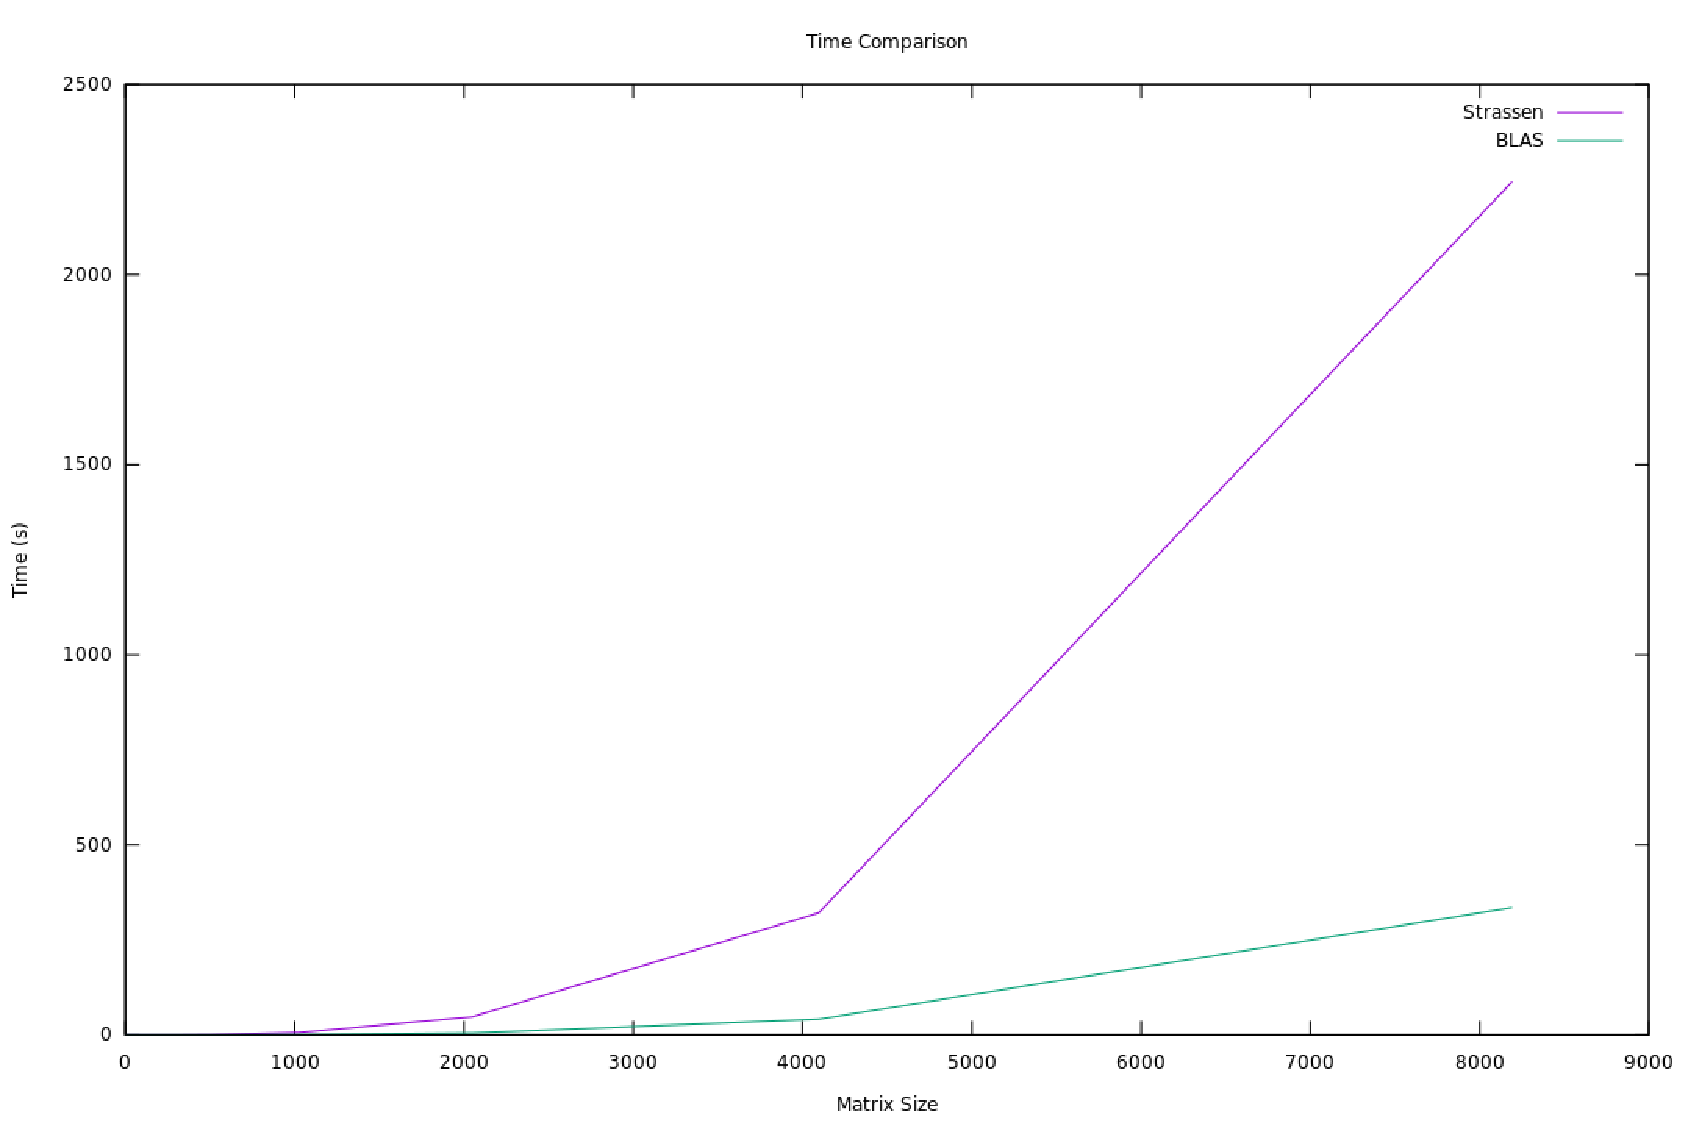
\includegraphics[width=1\linewidth]
{./figures/plot_time_no_opt.pdf}
\caption{Comparação do tempo gasto pelo método de Strassen com a biblioteca BLAS.} 
\label{time_test}
\end{figure}

Quando dizemos que o tempo gasto é $O(n^{\alpha})$, estamos dizendo que o tempo gasto $t$ é dado por:

\[
 t \approx C \times n^{\alpha} \Rightarrow log(t) \approx \alpha log(n) + log(C) ,
\]
onde $C$ é uma constante. Podemos portanto traçar os logaritmos para descobrir o expoente de fato do tempo gasto no teste.

\begin{figure}[H]
\centering
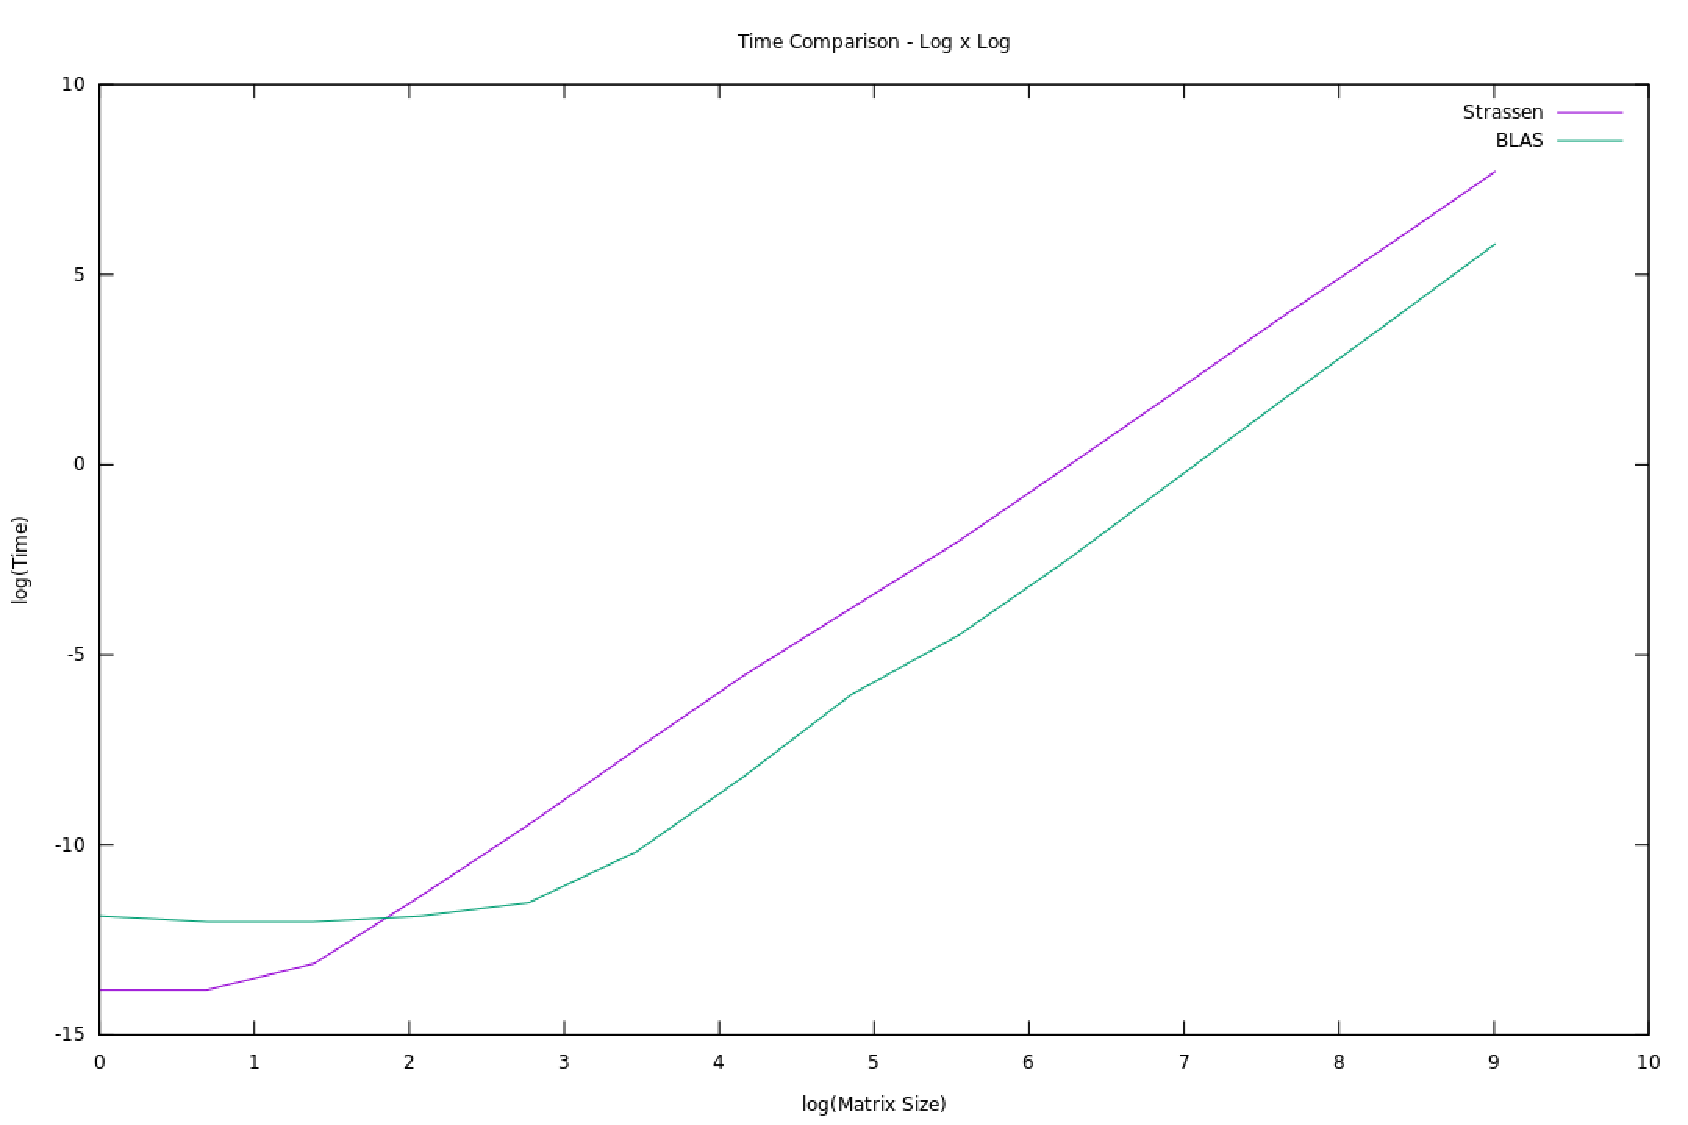
\includegraphics[width=1\linewidth]
{./figures/plot_time_no_opt_log.pdf}
\caption{Comparação do tempo gasto pelo método de Strassen com a biblioteca BLAS - log x log.} 
\label{time_test_log}
\end{figure}
 
Utilizando a função \emph{fit} do gnuplot, o coeficiente $\alpha_s$ para o método de Strassen
foi determinado como $\alpha_s = 2.71889$, enquanto que para o método implementado na BLAS foi obtido
$\alpha_b = 2.81103$. A diferença observada em relação ao teórico esperado provavelmente é devida a otimizações tanto do compilador
quanto da implementação da BLAS.

Ainda assim é possível observar que o expoente assintótico do método de Strassen é menor do que o obtido com a BLAS. Isto indica que existe um tamanho de matriz 
a partir do qual o método de Strassen será mais rápido.

\section*{Otimização do Método de Strassen}

Como a ineficiência do método de Strassen se manifesta mais explicitamente para matrizes pequenas, uma abordagem possível para acelerar o algoritmo seria estabelecer um
tamanho mínimo de bloco, a partir do qual o método seria substituído pelo algoritmo implementado na BLAS. Foi feito um teste para estabelecer qual ponto seria mais adequado para esta transição.

\begin{figure}[H]
\centering
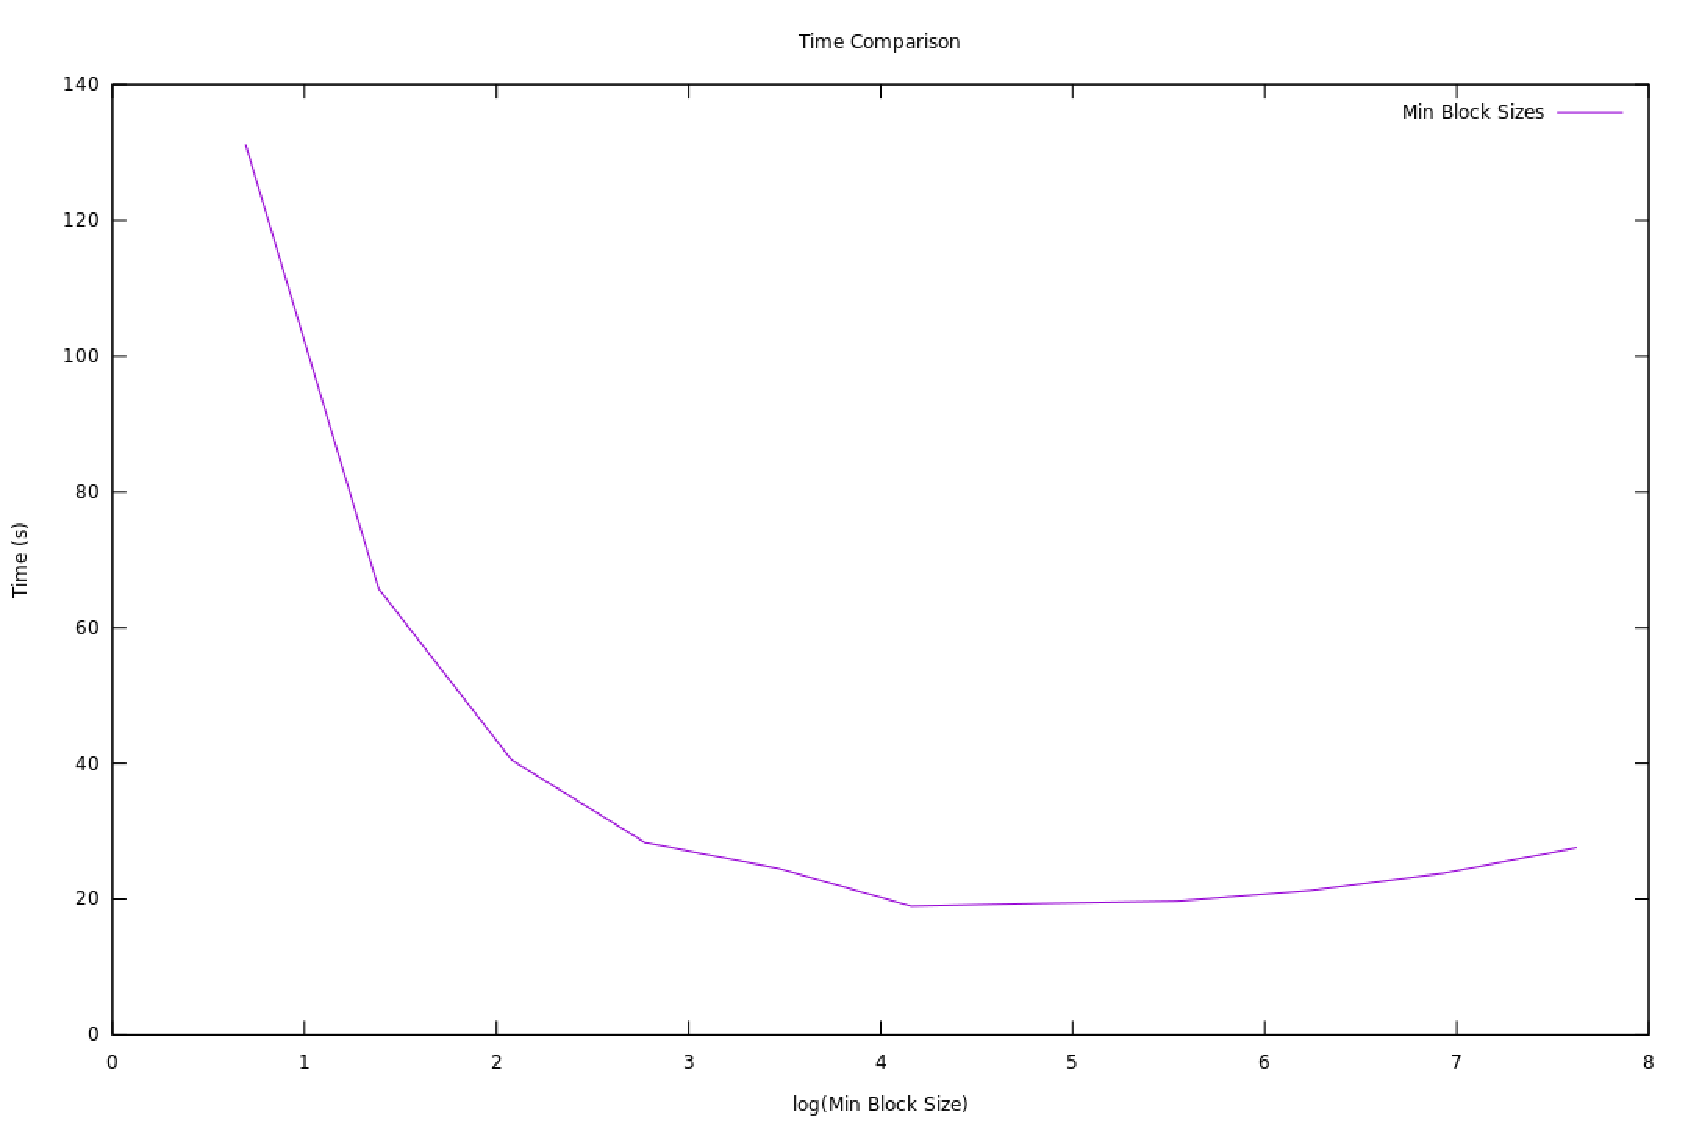
\includegraphics[width=1\linewidth]
{./figures/plot_block_test.pdf}
\caption{Comparação do tempo gasto pelo método de Strassen com diferentes tamanhos mínimos de bloco.} 
\label{block_test}
\end{figure}

O teste consistiu em medir o tempo gasto para multiplicar duas matrizes $4096 \times 4096$ com diferentes tamanhos
mínimos de bloco, a partir do qual se usaria a BLAS. O resultado obtido foi que o ótimo está em utilizar a BLAS para blocos com tamanho 
menor ou igual a $64$.



\section*{Comparação de Tempo com Método de Strassen Otimizado}

Finalmente, com o tamanho mínimo determinado pelo teste anterior, resta testar o tempo gasto pelo algoritmo com esta otimização.

\begin{figure}[H]
\centering
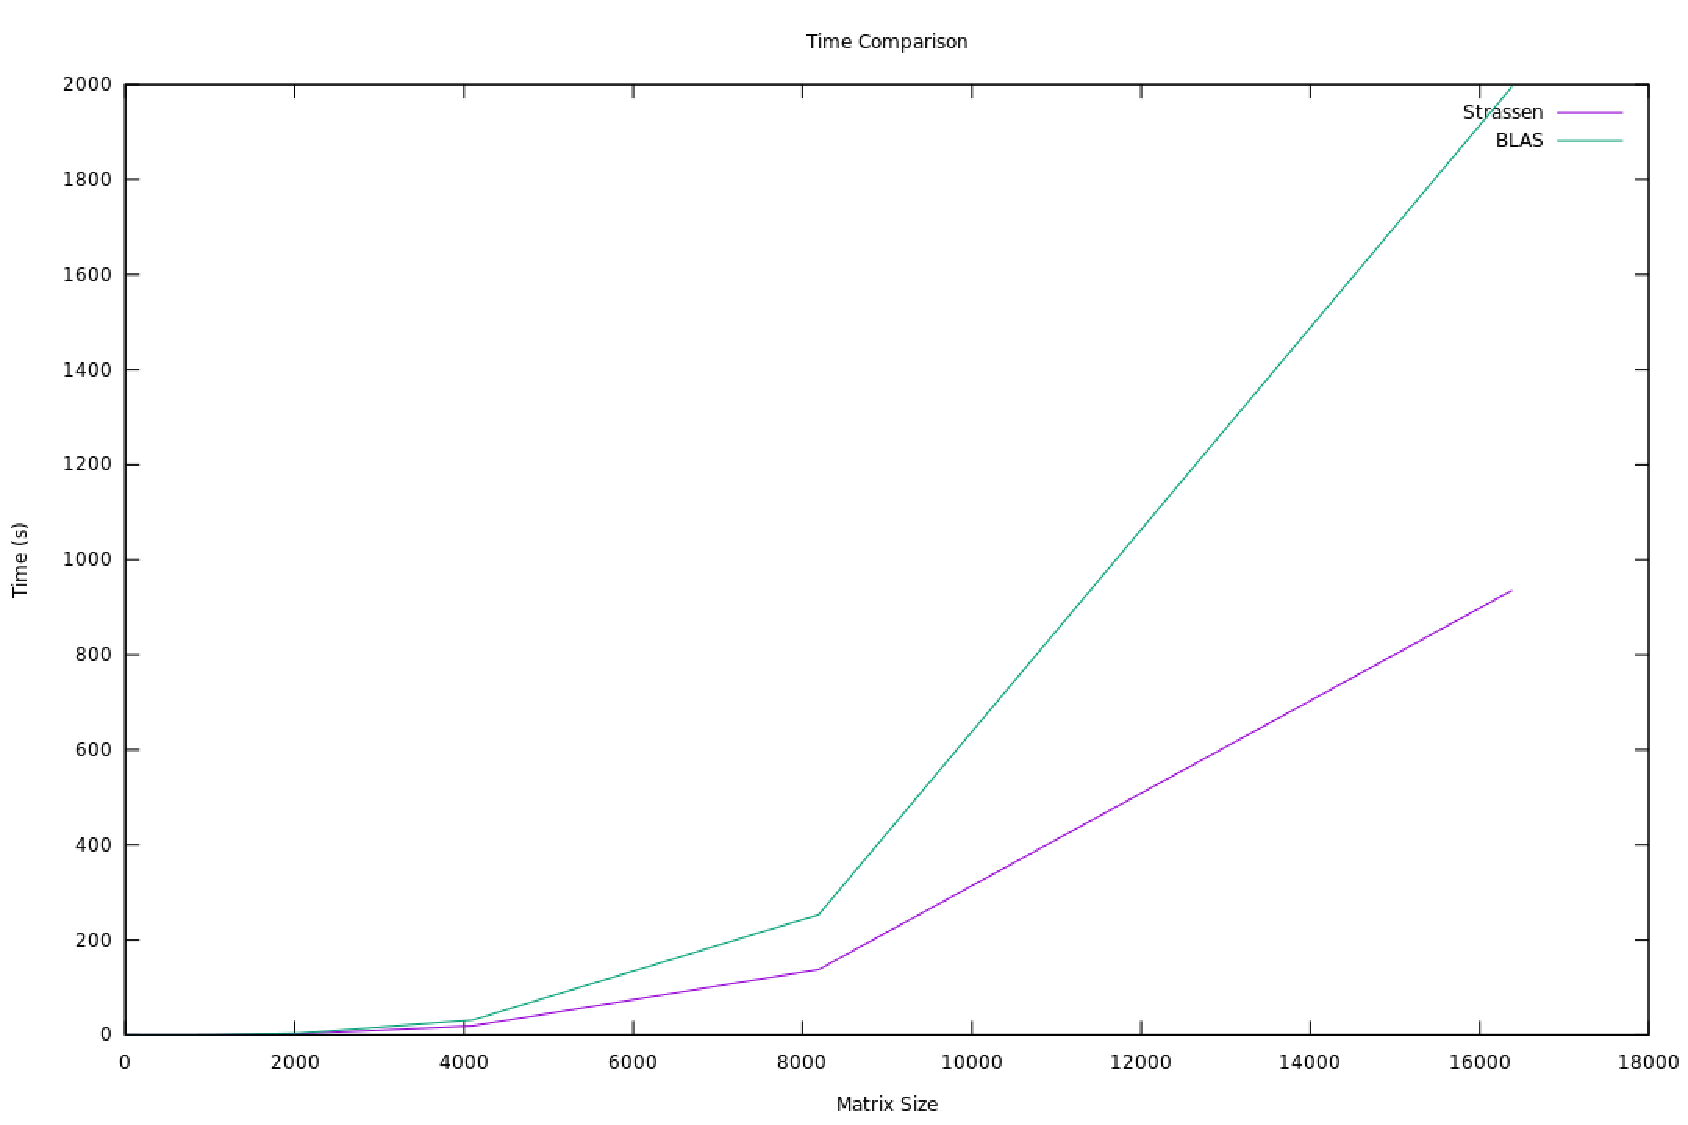
\includegraphics[width=1\linewidth]
{./figures/plot_time.pdf}
\caption{Comparação do tempo gasto pelo método de Strassen Otimizado com a implementação da BLAS.} 
\label{opt_time}
\end{figure}

Notamos que com esta configuração, o método de Strassen atinge um tempo melhor do que a implementação da BLAS para todos os tamanhos de matriz, sendo que,
claramente, o tempo para matrizes com tamanho menor do que o mínimo estipulado será igual para os dois tipos de solução.

\section*{Teste de Erro}

Foi avaliada ainda a razão entre a norma-$2$ da diferença entre o resultado obtido pelos métodos e a norma-$2$ da resposta da BLAS, já que a BLAS está validada por seu uso de muitos anos.
Naturalmente, para tamanhos menores que o bloco mínimo o erro foi da ordem do zero da máquina pois o mesmo cálculo foi executado. Fora isso, o erro se comporta como esperado,
crescendo com comportamento até menor que $O(n)$.

\begin{figure}[H]
\centering
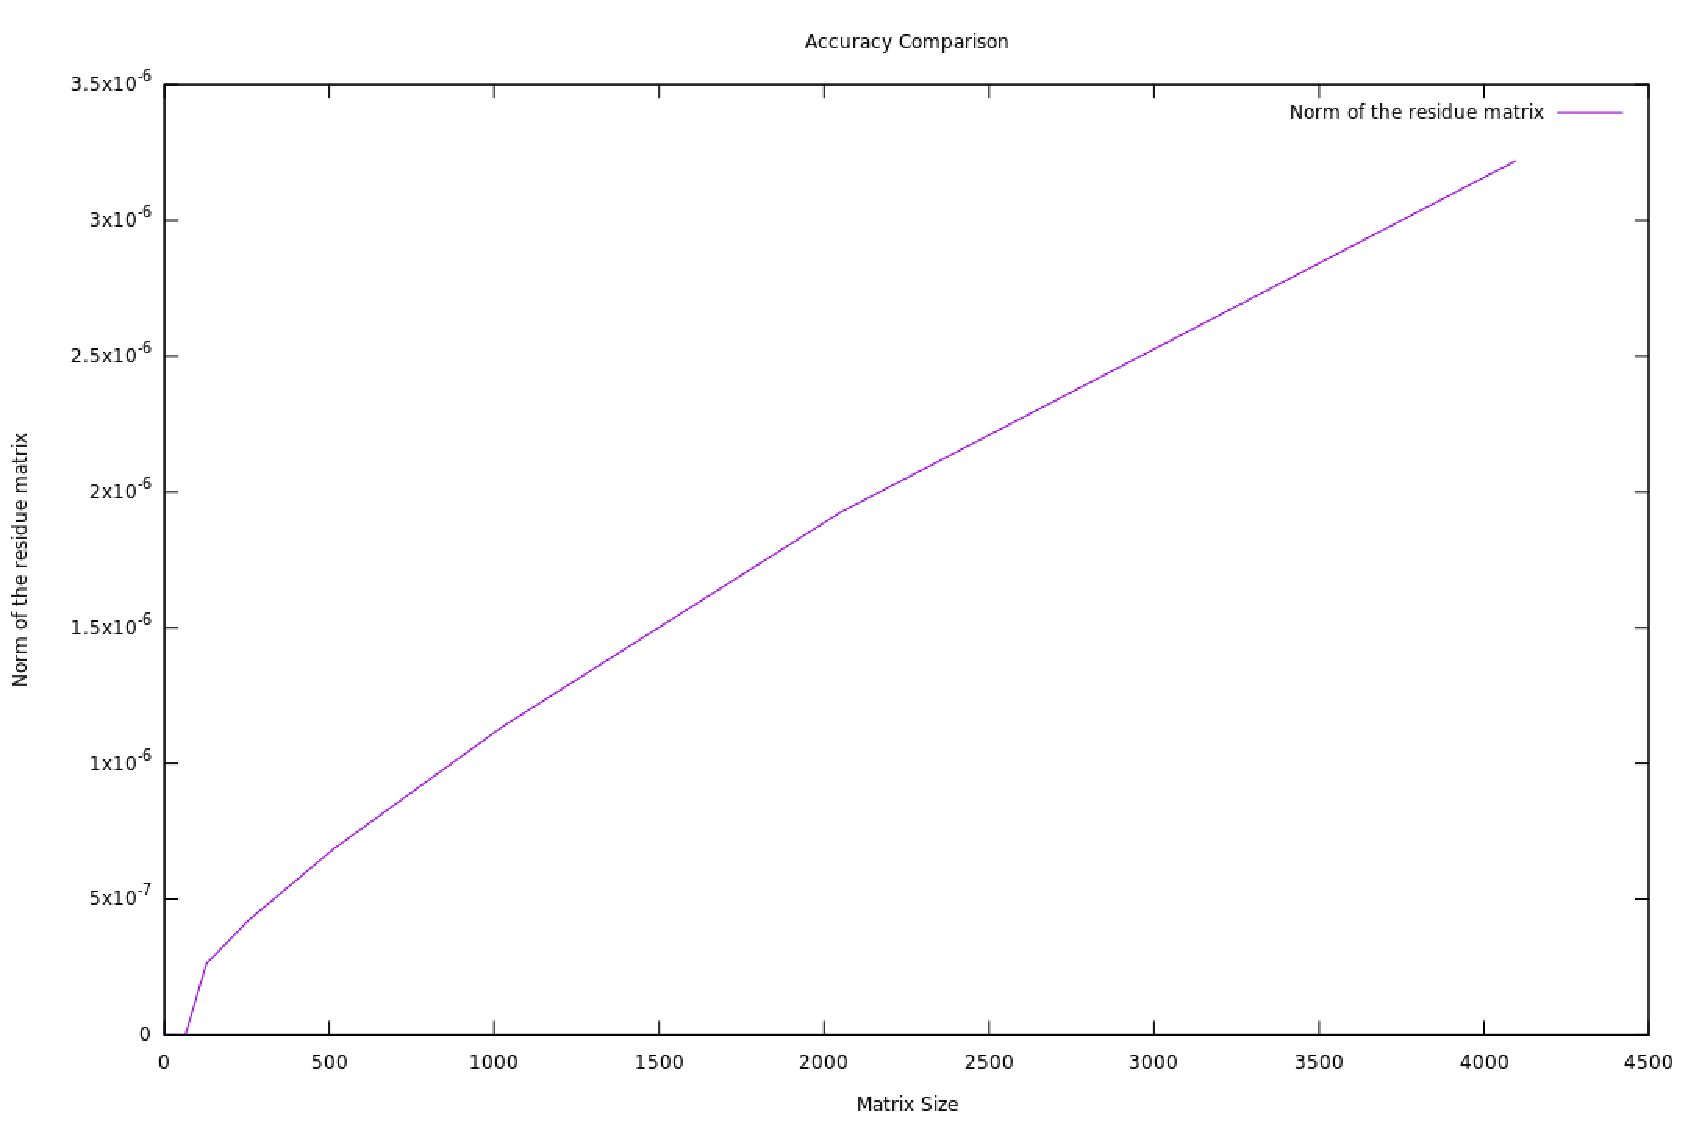
\includegraphics[width=1\linewidth]
{./figures/residue.pdf}
\caption{Norma do erro relativo obtido para o algoritmo de Strassen.} 
\label{residue}
\end{figure}

\section*{Sugestões para Melhoria do Estudo}

Em geral o resultado obtido foi dentro do esperado e satisfatório, entretanto há algumas otimizações encontradas na literatura que poderiam aumentar a performance do método.

Em particular, a implementação feita, para que seja compatível com a BLAS diretamente, exige que seja feita uma aritmética com os índices das submatrizes várias vezes durante
o método. Esta aritmética pode ser evitada se a matriz for expressa no \emph{array} de outra forma. Uma formulação que pareceu ter benefícios é a indexação de Morten \cite{Huang},
Onde a ordenação já respeita os blocos das submatrizes. Além de reduzir o número de operações, o acesso sequencial de memória causaria também uma melhoria, potencialmente grande,
da performance do código. 

Além disso, no caso em que as matrizes não são quadradas com tamanho da forma $2^n$ foi implementado um \emph{padding} que preenche a matriz com zeros até a próxima potência de 2.
Isto me parece ineficiente tanto em termos de alocação de memória quanto em termos de operações adicionadas. Seria interessante avaliar a técnica mencionada de pegar um bloco mínimo que
concentra os fatores que não sejam potências de $2$ para tentar achar uma forma melhor de preenchimento.

Outras técnicas de otimização aplicáveis neste caso seriam o \emph{loop unrolling} na criação das submatrizes e a implementação em paralelo, já que muitas operações não têm dependência sequencial.

\bibliography{bibliography}
\bibliographystyle{ieeetr}

\end{document}